\subsubsection{Running a CUDA program on a GPU}

The following section is dedicated to understanding the execution of the \dquotes{convolve} kernel on a fictitious dual-core GPU. In other words, we present an example of a kernel function execution (and therefore GPU-executed) that implements a convolution operation. It also aims to show why memory management is also fundamental inside the GPU.

\highspace
The kernel execution requirements for this explanation are:
\begin{itemize}
    \item Each \textbf{thread block} must execute \textbf{128 CUDA threads}.
    \item Each thread block must allocate $130 \times \texttt{sizeof(float)} = 520$ bytes of shared memory. In other words, \textbf{each thread block requires 520 bytes of shared memory}.
\end{itemize}
Let's take an array of size $N$ as \textbf{input} to the kernel function. When the kernel function is executed (launched), it generates thousands of thread blocks because the array size $N$ is assumed to be very large.

\begin{lstlisting}[language=C++]
#define THREADS_PER_BLK 128
convolve<<<(N/THREADS_PER_BLK), THREADS_PER_BLK>>>(N, input_array, output_array);
\end{lstlisting}

\noindent
Where:
\begin{itemize}
    \item \texttt{N/THREADS\_PER\_BLK} is the number of blocks per grid.
    \item \texttt{THREADS\_PER\_BLK} is the number of threads per block, 128 CUDA threads in our case.
\end{itemize}
The \textbf{main task} of the \emph{GPU Work Scheduler} is to \textbf{manage the two available cores} (let's say Core 0 and Core 1), where each core has its own \textbf{Fetch/Decode units}, \textbf{execution context storage} for 384 CUDA threads (12 warps), and \textbf{shared memory storage} (1.5 KB).

\highspace
Note that this architecture has fictitious cores that are smaller than V100 SM cores, with fewer execution units, less support for active warps, and less shared memory.

\begin{figure}[!htp]
    \centering
    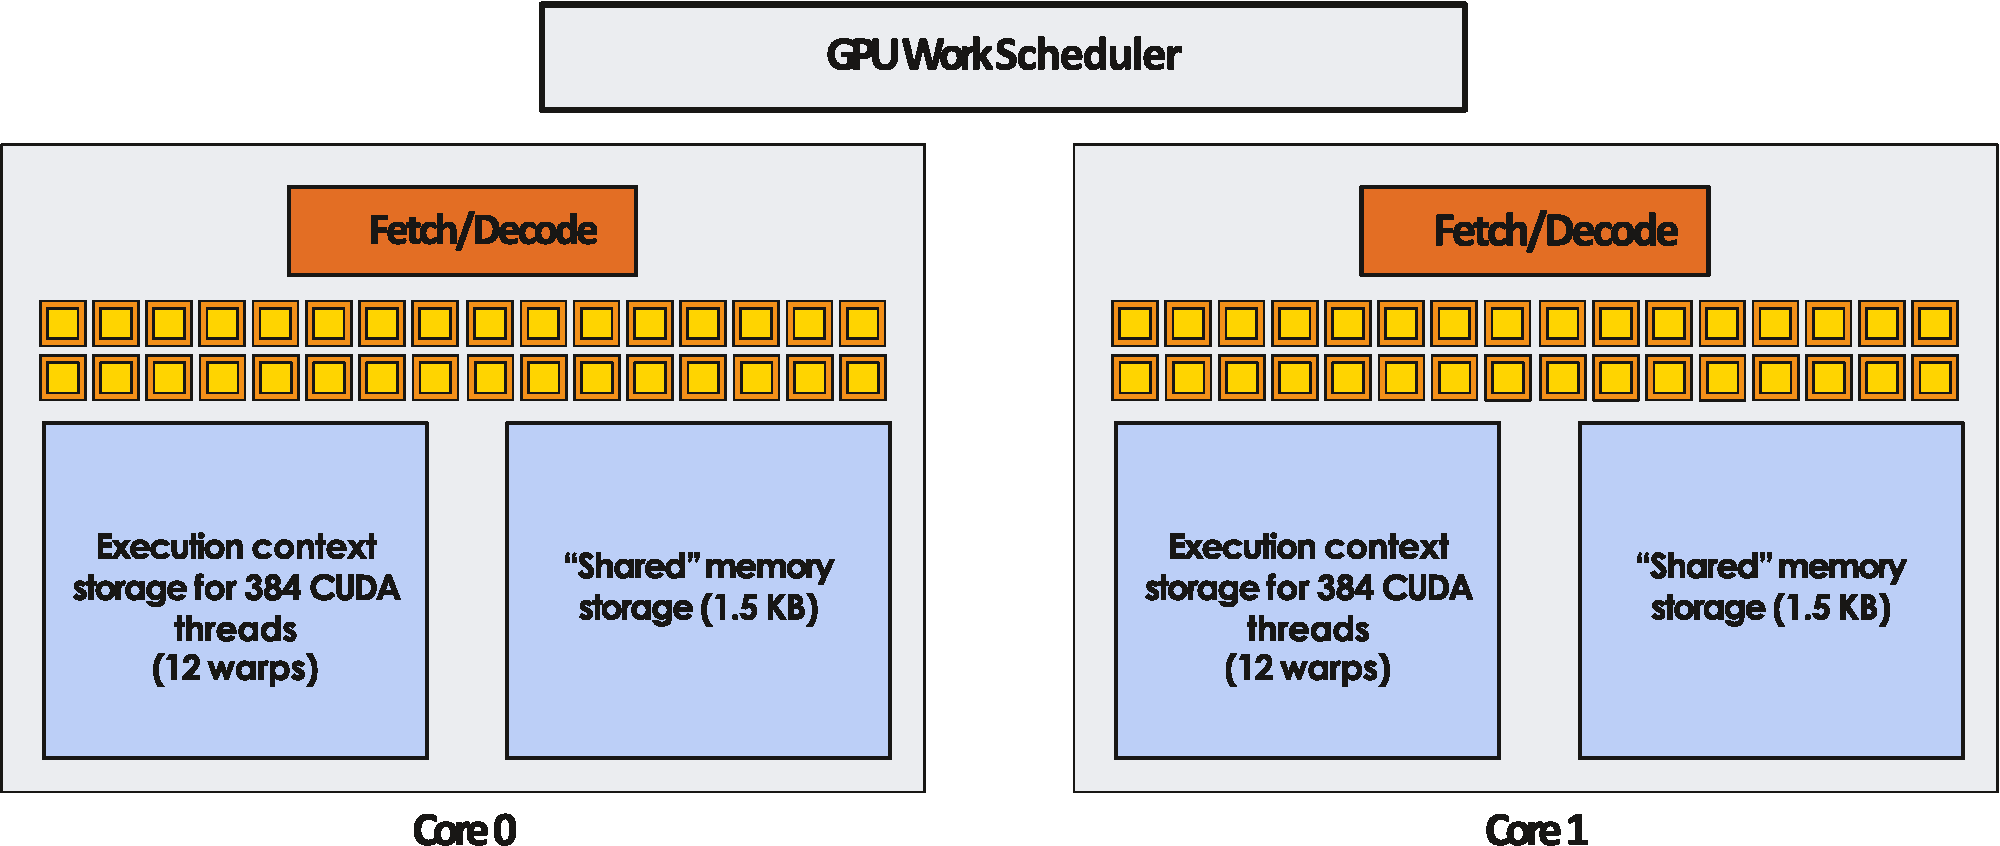
\includegraphics[width=\textwidth]{img/cuda-convolve-kernel-1.pdf}
\end{figure}

\newpage

\begin{flushleft}
    \textcolor{Green3}{\faIcon{tachometer-alt} \textbf{Execution}}
\end{flushleft}
\begin{enumerate}
    \item The \textbf{host} (CPU) \textbf{sends a command to the CUDA device} (GPU), which is the execution of the kernel function.
    \begin{itemize}
        \item \textbf{Execute}: convolve (kernel function)
        \item \textbf{Args}:
        \begin{itemize}
            \item \texttt{N} $= 128'000$
            \item \texttt{input\_array}
            \item \texttt{output\_array}
        \end{itemize}
        \item \textbf{Number of blocks}: 1000. Note that the number of blocks is given by the formula:
        \begin{equation*}
            \dfrac{
                \texttt{N}
            }{
                \texttt{THREADS\_PER\_BLK}
            }
        \end{equation*}
        Therefore, the size of the array is easily calculated as:
        \begin{equation*}
            \dfrac{\texttt{N}}{128} = 1000 \: \Rightarrow \: \texttt{N} = 128 \times 1000 = 128'000
        \end{equation*}
    \end{itemize}


    \item The \emph{scheduler} maps \emph{block 0} to \emph{Core 0}, reserving execution contexts for 128 threads and 520 bytes of shared memory to meet requirements.
    \begin{figure}[!htp]
        \centering
        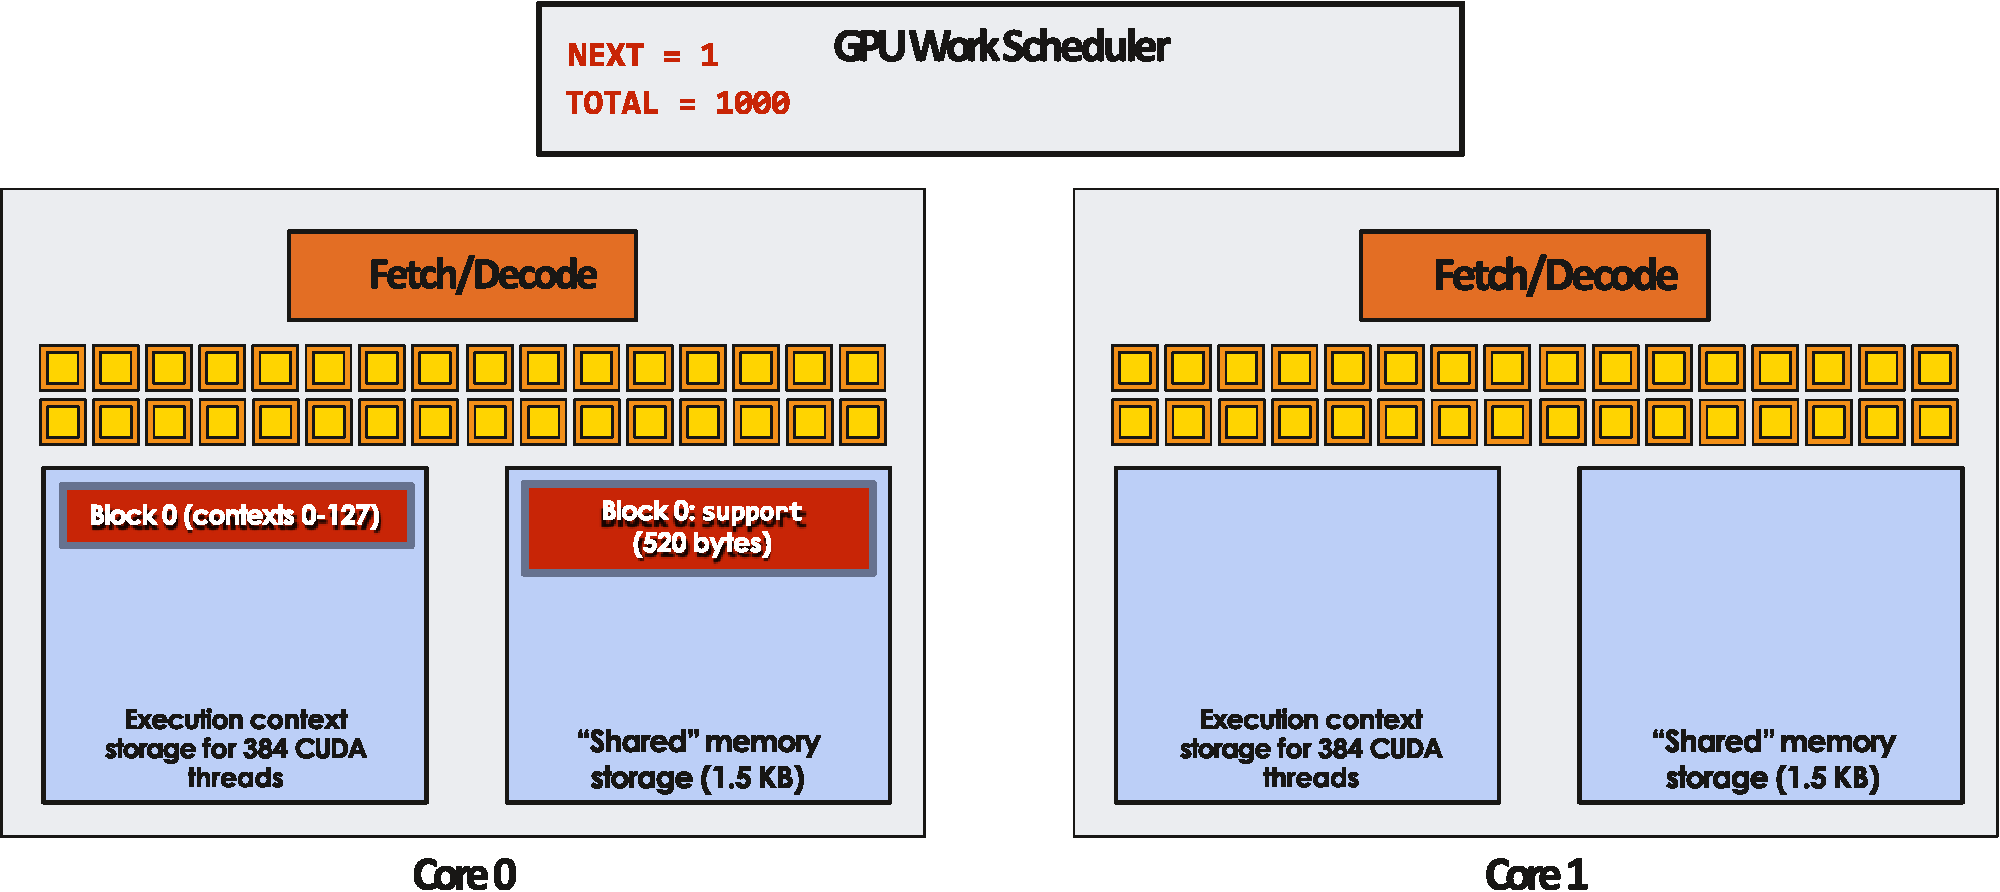
\includegraphics[width=\textwidth]{img/cuda-convolve-kernel-2.pdf}
    \end{figure}

    \newpage

    \item The \emph{scheduler} continues to map blocks to available execution contexts, so it now maps \emph{block 1} to \emph{Core 1}. This shows \textbf{interleaved mapping} (where the scheduler maps blocks to available execution contexts across different cores, ensuring efficient use of resources).\index{CUDA Interleaved Mapping}
    \begin{figure}[!htp]
        \centering
        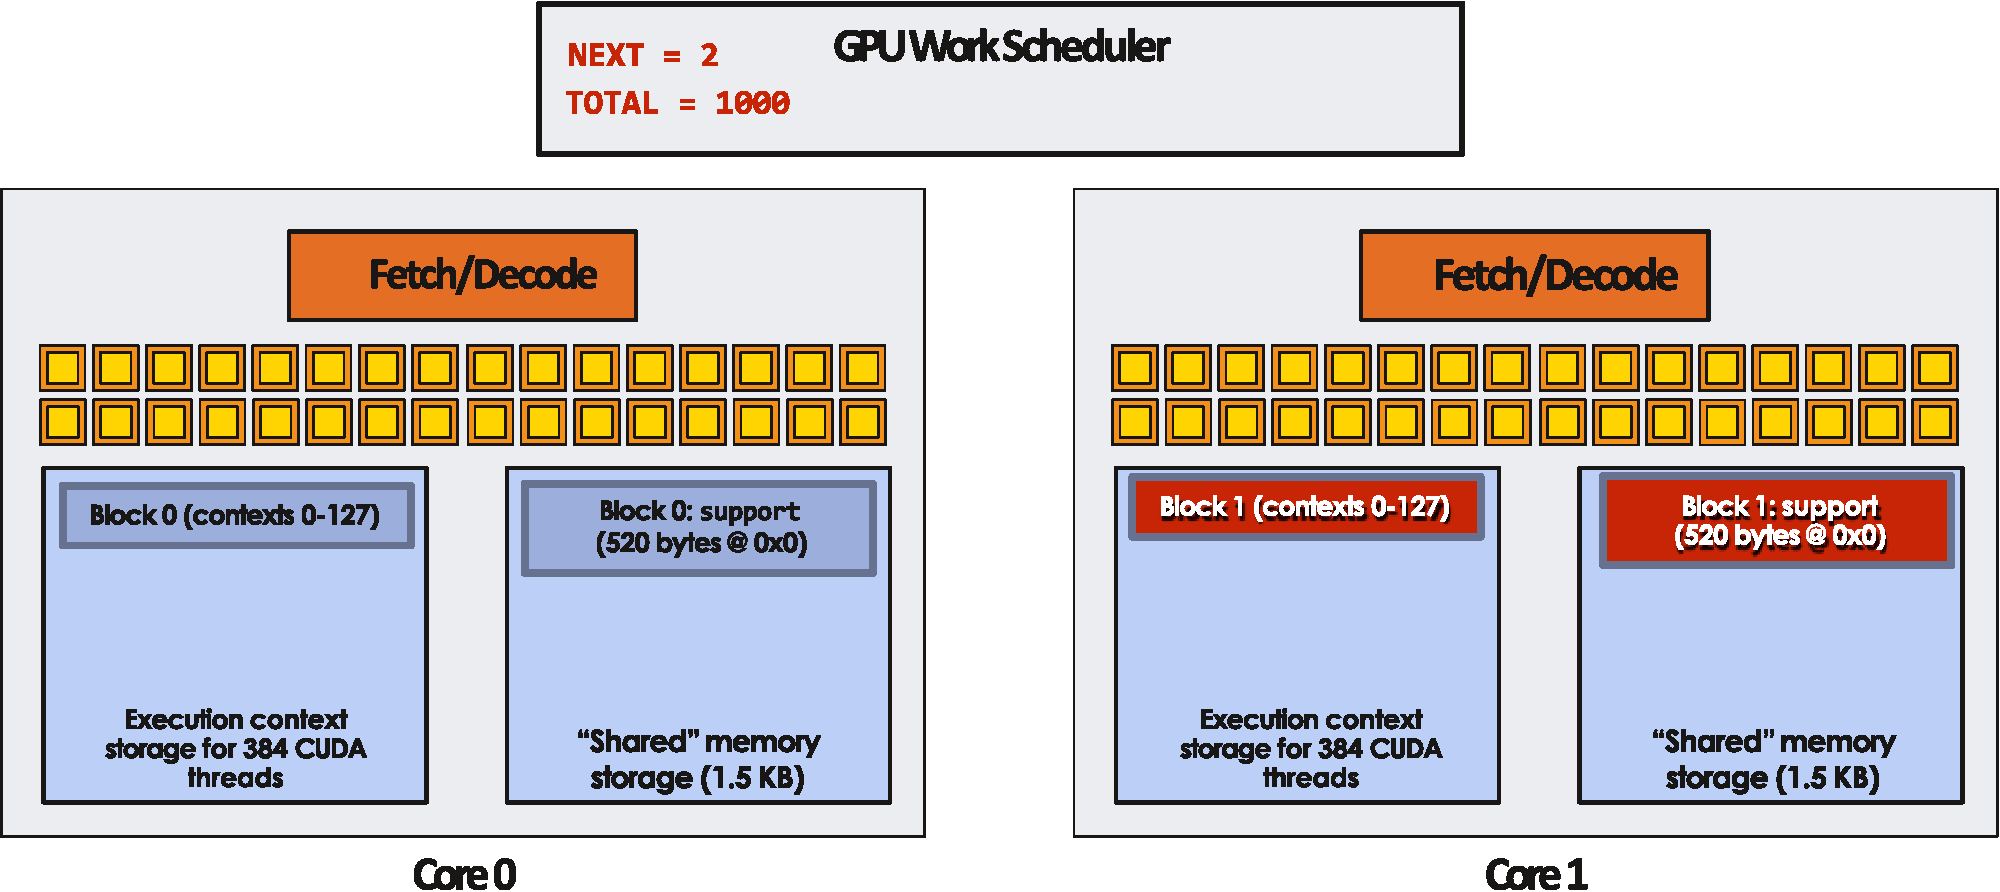
\includegraphics[width=\textwidth]{img/cuda-convolve-kernel-3.pdf}
    \end{figure}


    \item As in the previous step, there is a interleaved mapping phenomena. The scheduler maps \emph{block 2} to \emph{Core 0}. But now the shared memory (\emph{Core 0}) is saturated because three concurrent blocks allocate $520 \texttt{ bytes} \times 3 = 1.56 \texttt{ KB} > \text{limit } (1.5 \texttt{ KB})$.
    \begin{figure}[!htp]
        \centering
        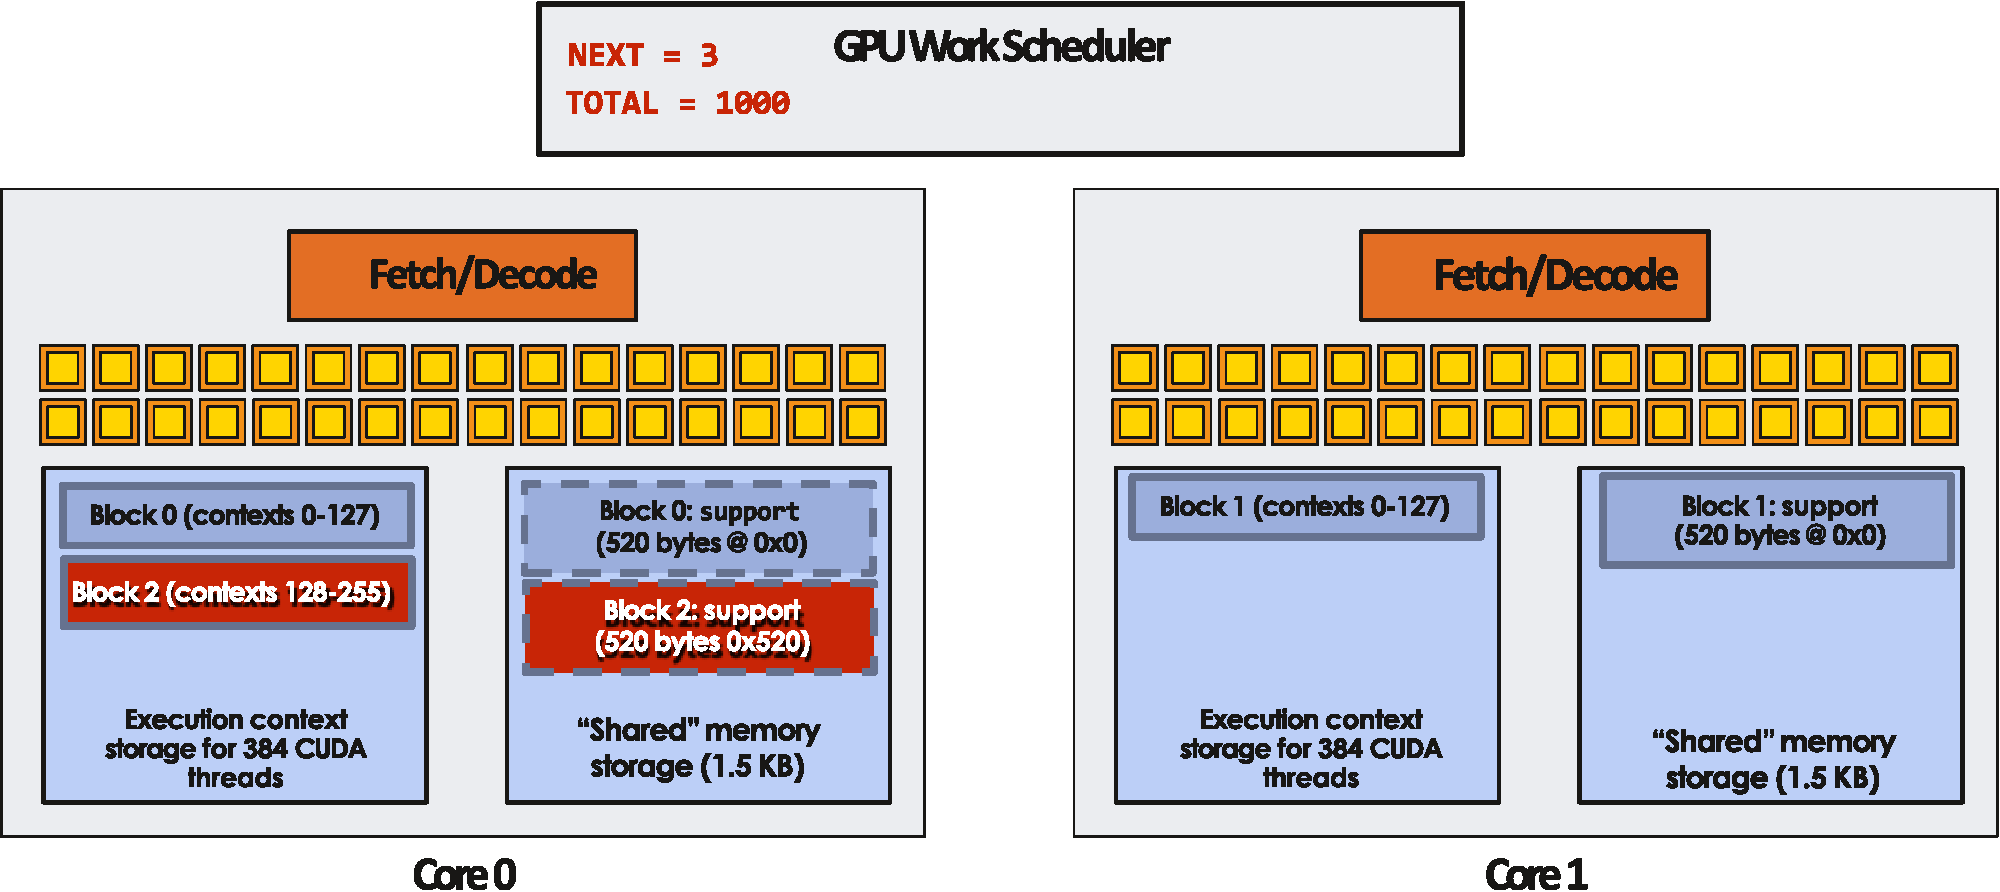
\includegraphics[width=\textwidth]{img/cuda-convolve-kernel-4.pdf}
    \end{figure}

    \newpage

    \item The scheduler assigns \emph{block 3} to \emph{Core 1}. But now the shared memory of \emph{Core 1} is also \textbf{saturated}, because three concurrent blocks allocate $520 \texttt{ bytes} \times 3 = 1.5 \texttt{ KB} > \text{limit } (1.5 \texttt{ KB})$. So we can say that only two thread blocks fit on one core.
    \begin{figure}[!htp]
        \centering
        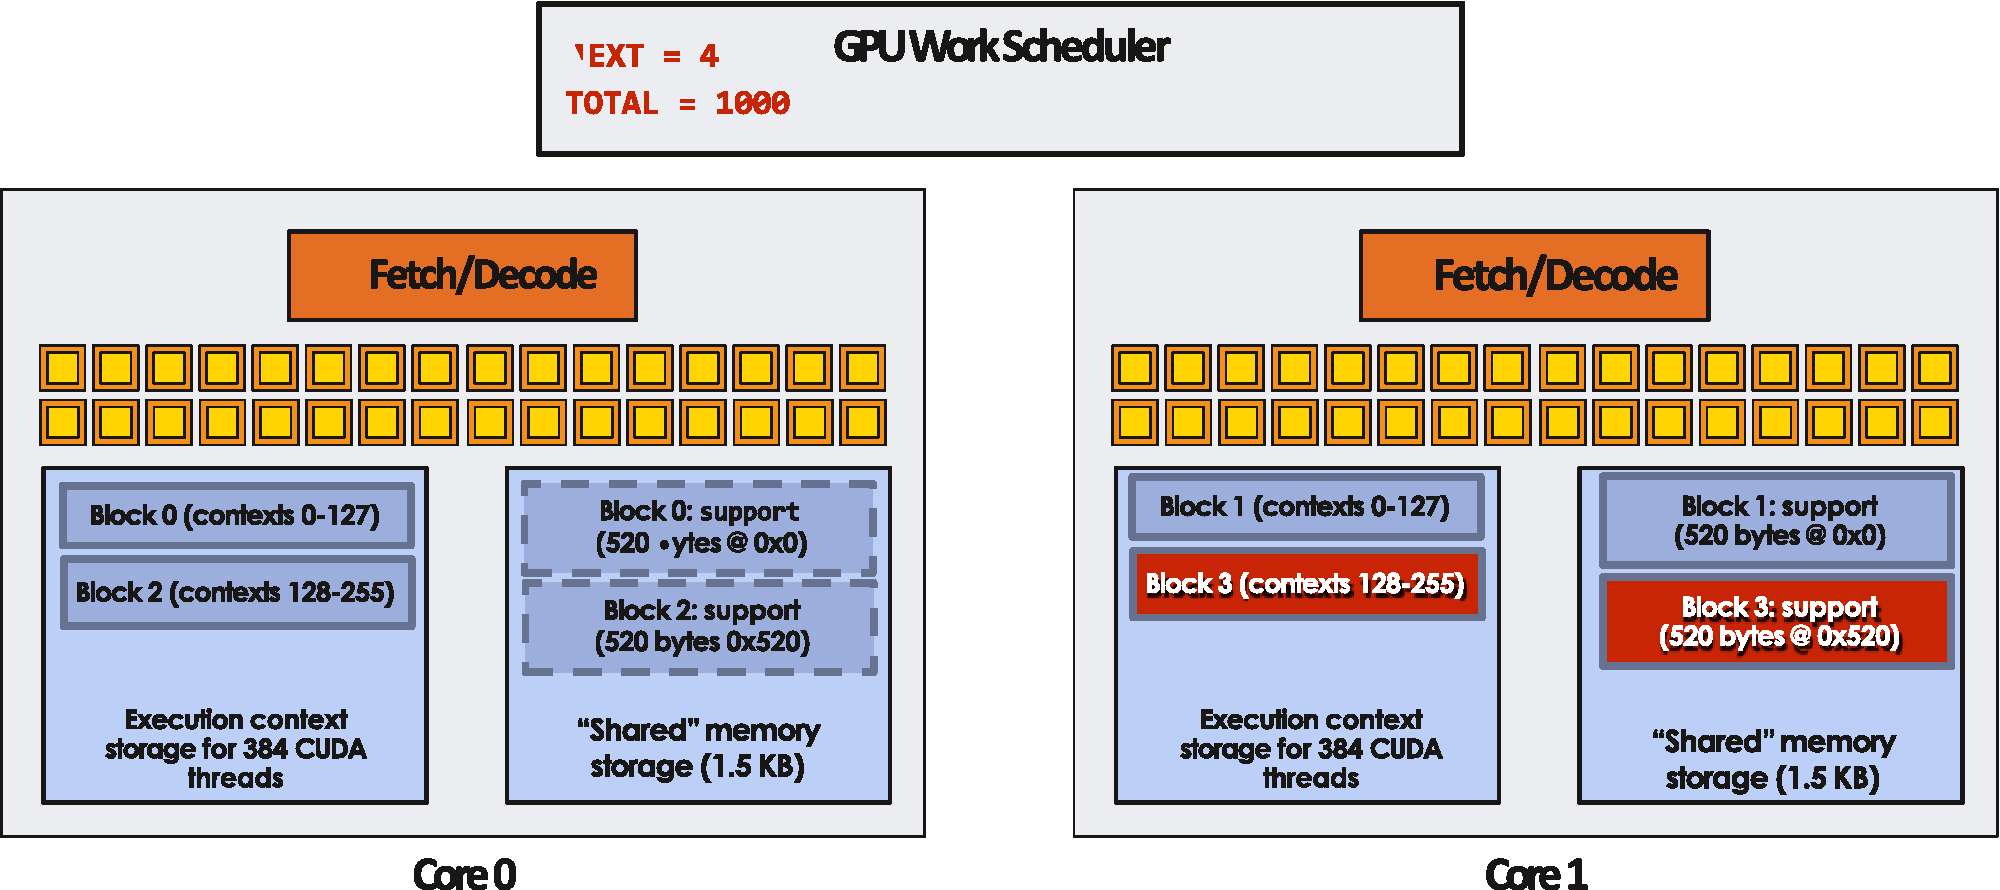
\includegraphics[width=\textwidth]{img/cuda-convolve-kernel-5.pdf}
    \end{figure}

    \item The scheduler waits for a task to complete on a block. The following figure shows \emph{block 0} completing on \emph{Core 0}. Now \emph{Core 0} is ready to host execution blocks again.
    \begin{figure}[!htp]
        \centering
        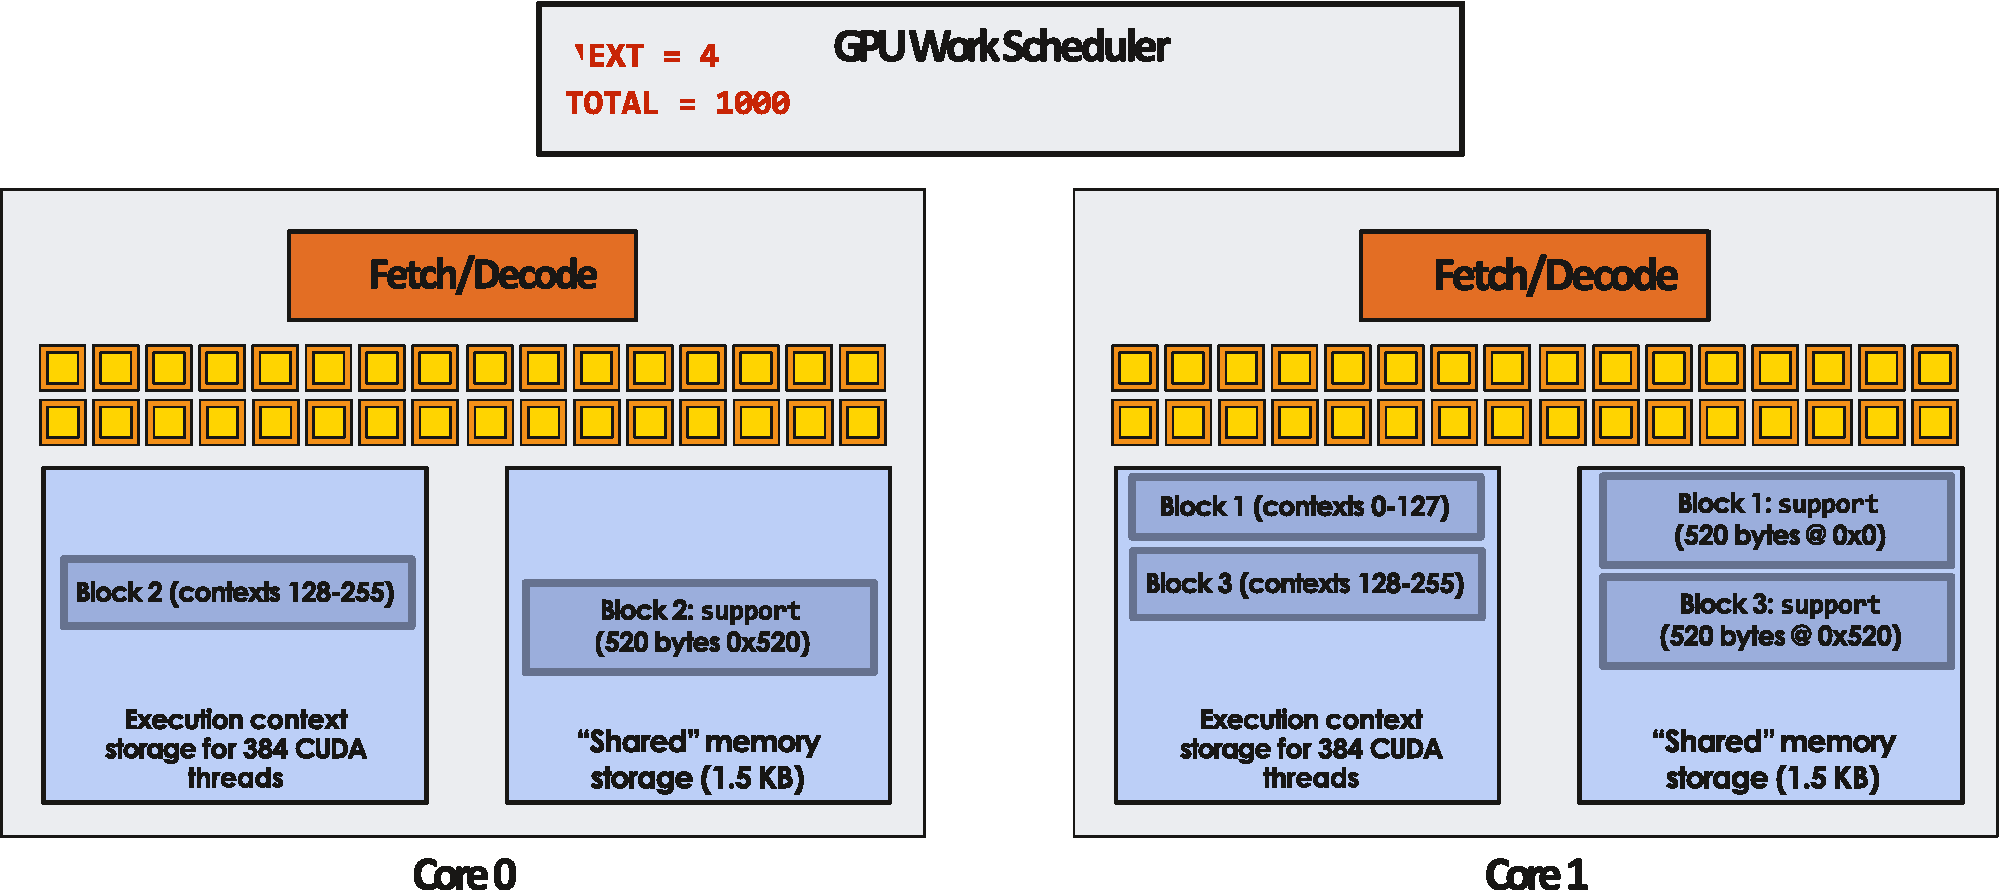
\includegraphics[width=\textwidth]{img/cuda-convolve-kernel-6.pdf}
    \end{figure}

    \newpage

    \item When the task is complete, the scheduler assigns \emph{block 4} to \emph{Core 0}.
    \begin{figure}[!htp]
        \centering
        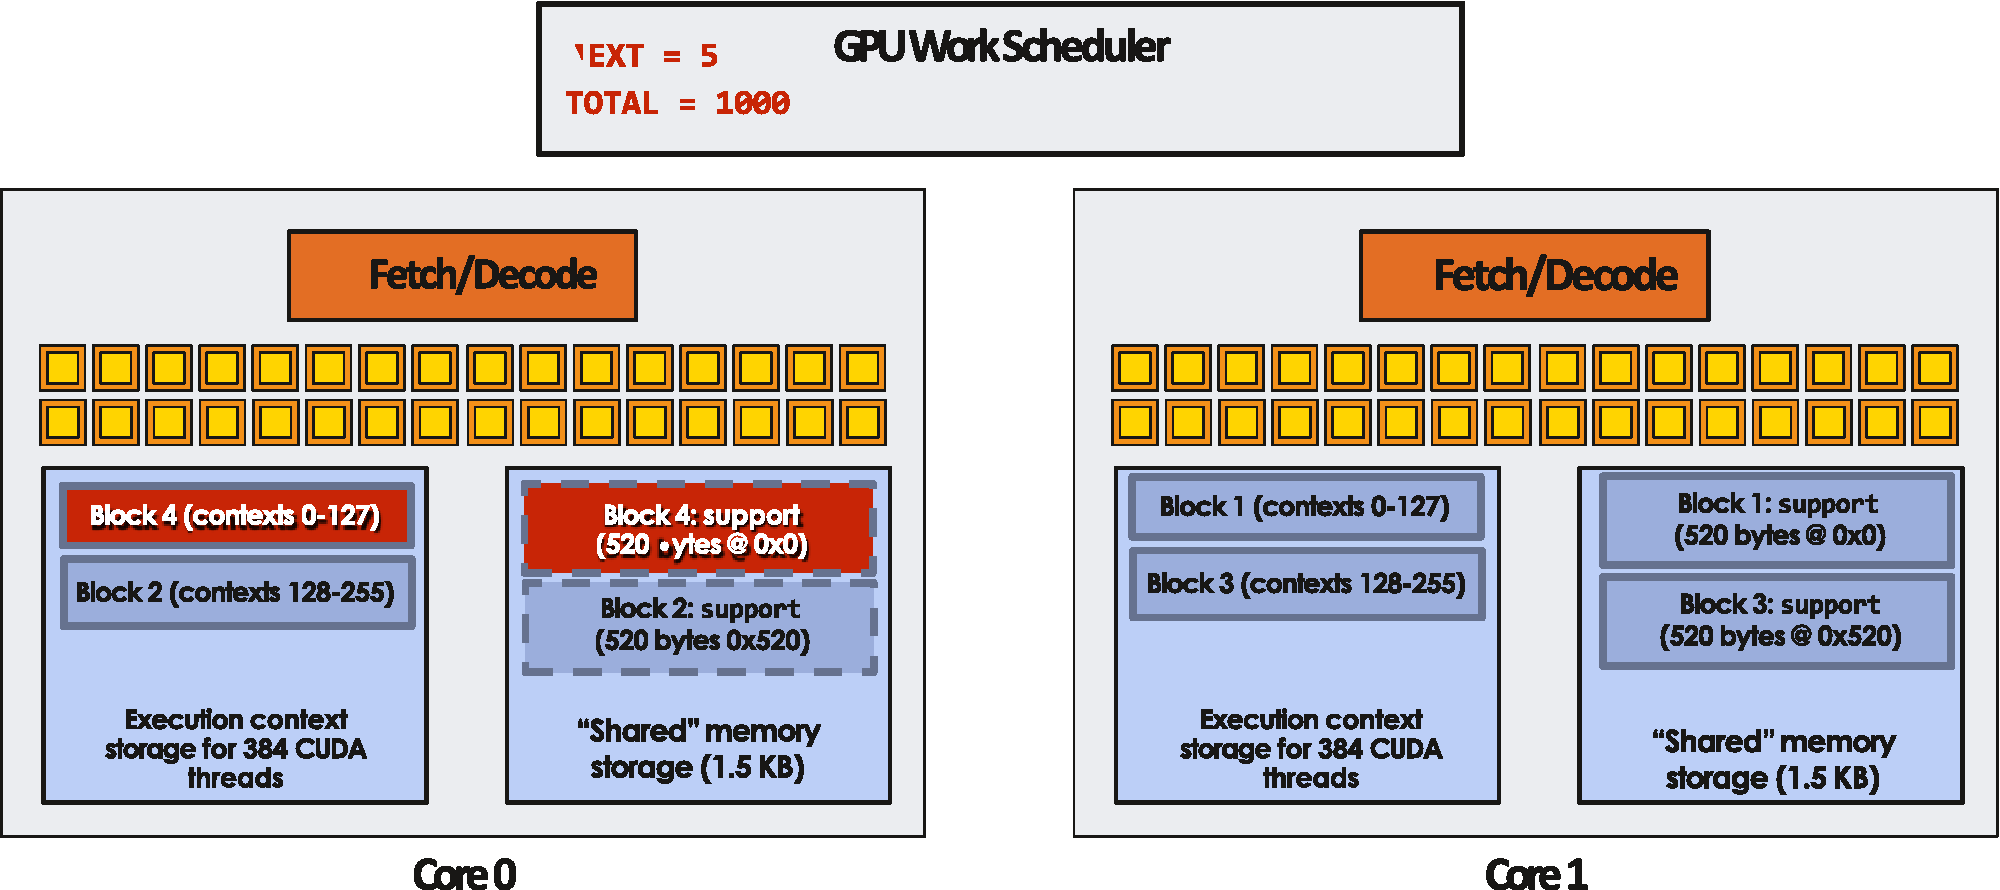
\includegraphics[width=\textwidth]{img/cuda-convolve-kernel-7.pdf}
    \end{figure}

    \item Thread \emph{block 2} completes on \emph{Core 0}.
    \begin{figure}[!htp]
        \centering
        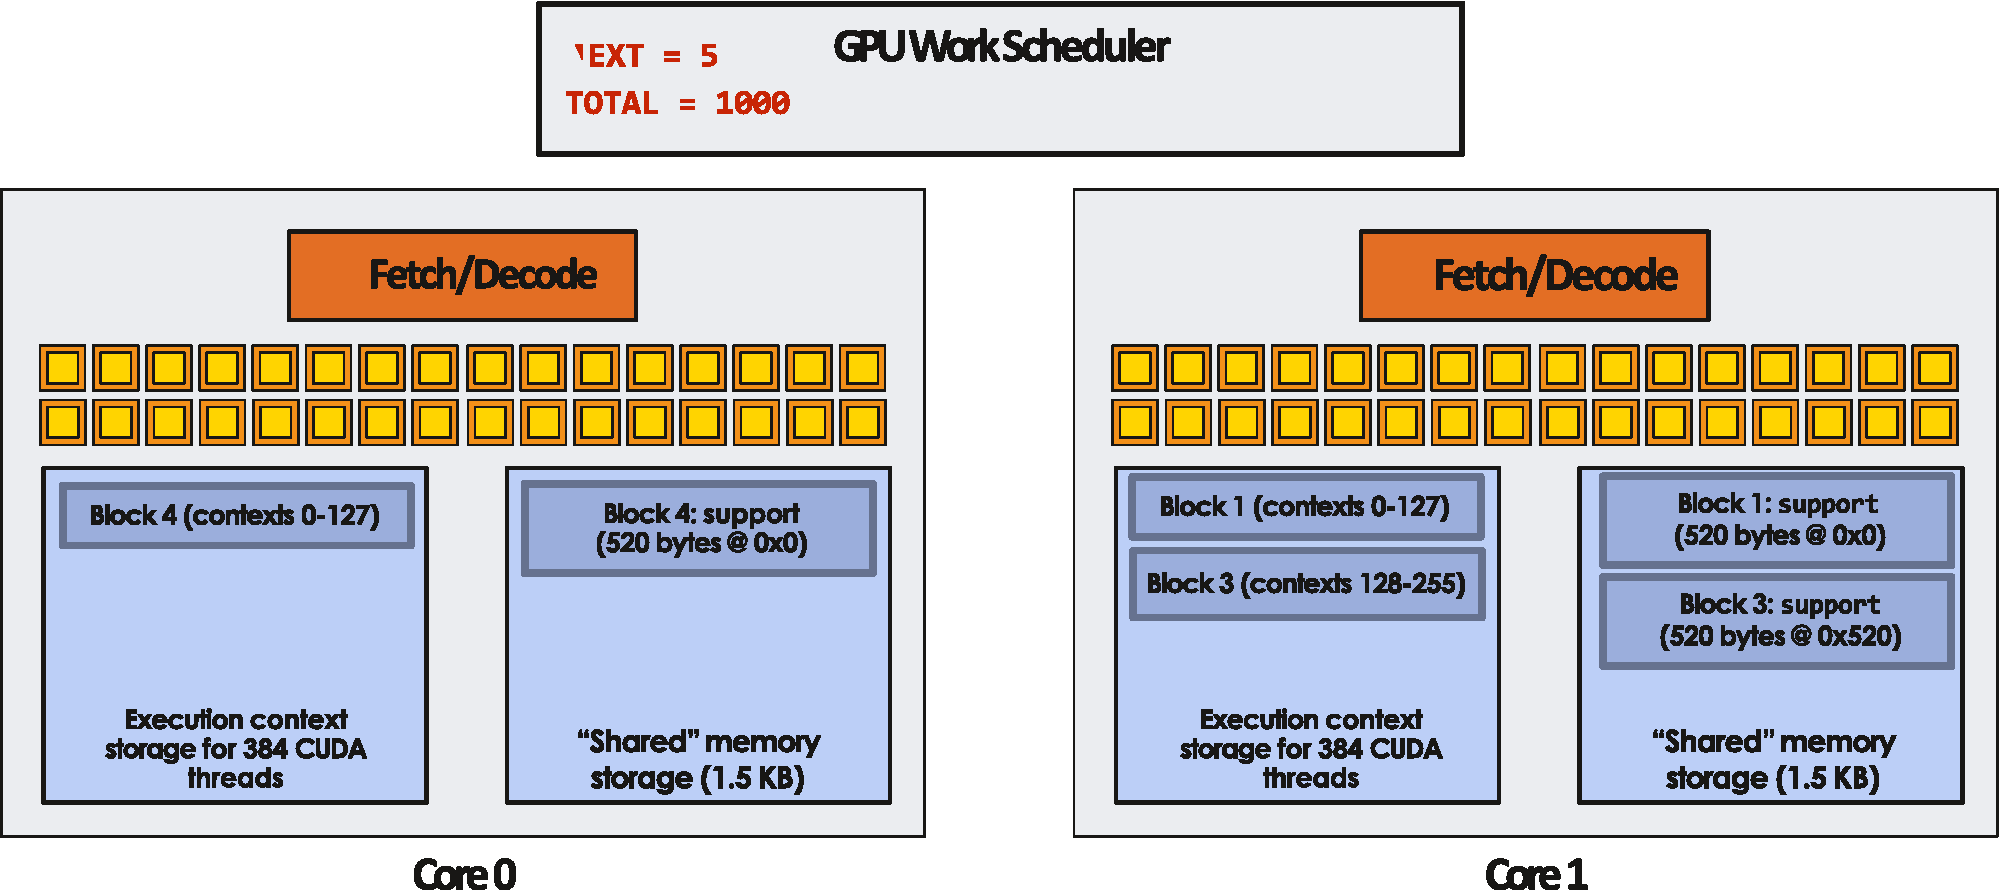
\includegraphics[width=\textwidth]{img/cuda-convolve-kernel-8.pdf}
    \end{figure}

    \item Finally, thread \emph{block 5} is scheduled on \emph{Core 0}.
    \begin{figure}[!htp]
        \centering
        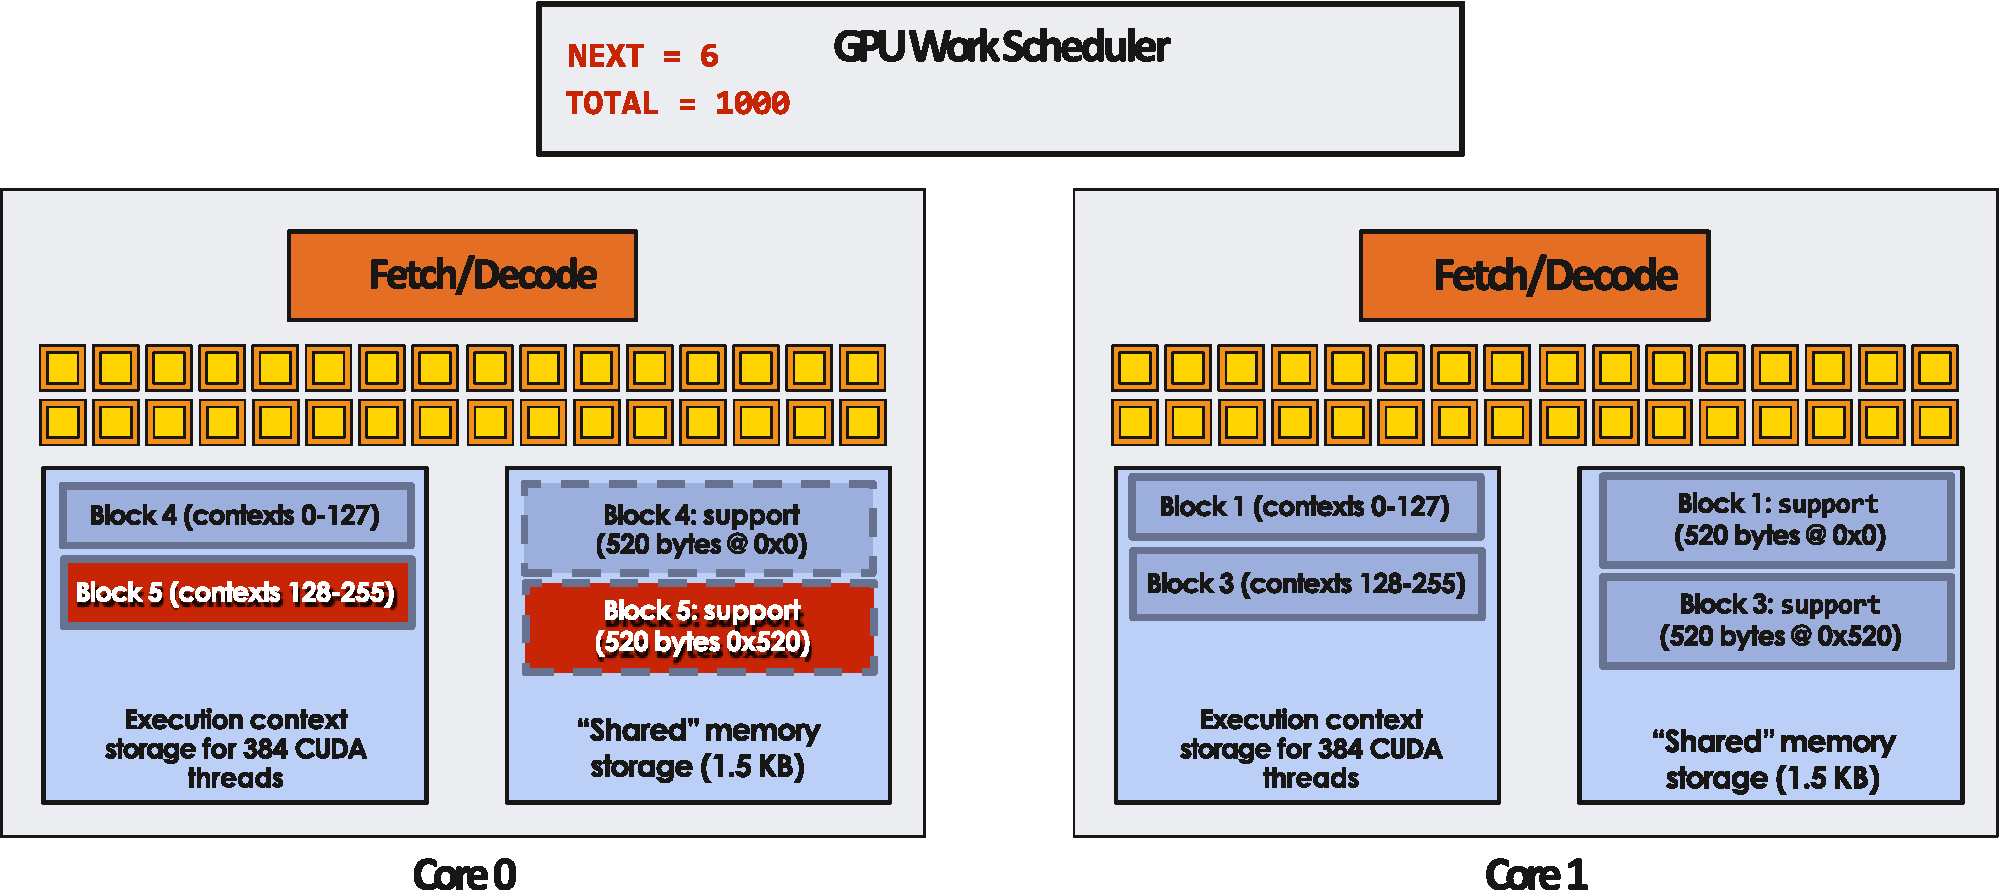
\includegraphics[width=\textwidth]{img/cuda-convolve-kernel-9.pdf}
    \end{figure}
\end{enumerate}
The explanation is intended to illustrate a phenomenon where the GPU scheduler has to manage limited shared memory resources across multiple thread blocks.
\begin{itemize}
    \item \textbf{Shared Memory Saturation}: When a GPU core's shared memory is fully occupied by existing thread blocks, new thread blocks cannot be scheduled until sufficient shared memory is freed up by the completion of some of the current thread blocks.
    
    \item \textbf{Idle Periods}: While the scheduler is waiting for shared memory to become available, the GPU cores may be idle. This doesn't mean the entire GPU is idle, but certain cores may not have new blocks to execute until resources are freed up.

    \item \textbf{Resource Contention}: This example shows how shared memory contention can affect the scheduling efficiency of a GPU. Efficient use of shared memory is critical to maximizing GPU performance.

    \item \textbf{Famous Phenomenon}: The concept of resource contention, whether it be shared memory, registers or other resources, is well known in parallel computing and GPU programming. It highlights the importance of optimizing memory usage to avoid bottlenecks and ensure efficient execution.
\end{itemize}
The example demonstrates how GPUs must juggle limited resources while maximizing throughput, a key aspect of parallel computing. By showing that the scheduler must wait before allocating new blocks, it emphasizes the importance of careful resource management in kernel design and execution.
